\documentclass[journal]{IEEEtran}
\usepackage{graphicx}
\usepackage[utf8]{inputenc}
\usepackage{float}
\ifCLASSINFOpdf
\else
\fi
\hyphenation{op-tical net-works semi-conduc-tor}
\begin{document}
\title{Generador de Kakuros}
\author{Eduard~Torres~Chaves,~\IEEEmembership{}
        y~Juan~José~Solano~Quesada,~\IEEEmembership{}
\thanks{E. Torres Chaves estudiante de Ingeniería en computación, Instituto Tecnológico de Costa Rica}% <-this % stops a space
\thanks{J.J. Solano estudiante de Ingeniería en computación, Instituto Tecnológico de Costa Rica}% <-this % stops a space
\thanks{}}
\maketitle
\begin{abstract}
This document discusses the study of the order of functions of pruning, backtracking and the functions in charge of permuting a list. It begins with the study of the large backtracking O and backtracking itself, then follows the study of the or the functions in charge of pruning and then the function in charge of performing permutations.

\end{abstract}
\begin{IEEEkeywords}
Backtracking, thread, poda.
\end{IEEEkeywords}
\IEEEpeerreviewmaketitle

\section{Introducción}
Un kakuro es un juego matemático que consiste en un conjunto de casillas blancas y negras, en las cuales se deben rellenar las casillas blancas en el tablero con números del 1 al 9 tal que las suma de los valores en las casilla sea igual a la clave que se encuentra a la izquierda para las filas y por encima de las columnas.\\
Entre sus reglas se distinguen que no se puede repetir el valor de una casilla en la misma fila y columna hasta que haya un espacio negro y, por ende, la cantidad máxima de celdas consecutivas es 9.\\
Los problemas matemáticos que representan estos enigmas pueden resolverse utilizando tecnicas de matriz matemática y backtracking.

\begin{figure}[h] 
        \centering 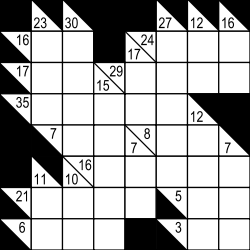
\includegraphics[width=.35\columnwidth]{kakuro_blank.png}
        \caption{
                \label{fig:samplesetup}
                Ejemplo de kakuro sin resolver
        }
\end{figure}

\begin{figure}[h] 
        \centering 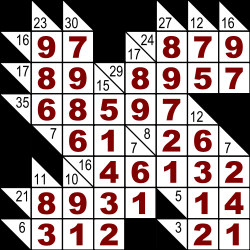
\includegraphics[width=.35\columnwidth]{kakuro_solved.png}
        \caption{
                \label{fig:samplesetup}
                Ejemplo de kakuro resuelto
        }
\end{figure}

\section{Análisis}
\subsection{Permutaciones}
En la figura 3
, se muestra la funci\'{o}n utilizada para calcular las permutaciones de una lista de tama\~{n}o $n$,  al estudiar la funci\'{o}n y las caracteristicas del mismo, se llega a la comclusion de que posee un orden de $\mathcal{O}(n!)$, ya que en la definici\'{o}n fundamental de una permutaci\'{o}n es la igual al orden del factorial de n o $!n$, este representa el número de formas distintas de ordenar $n$ objetos de manera diferente(sin repetir ordenes).El contenido de la lista se vuelve indiferente ya que, no importa el valor de los mismo a la hora de correr el algoritmo, pero si afecta el numero de los mismo.
\begin{figure}[hb] 
	\centering 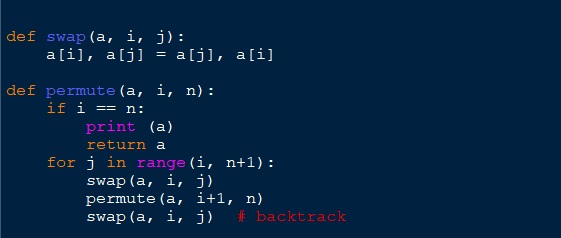
\includegraphics[width=0.9\columnwidth]{permutacion.png}
	\caption{
		\label{fig:samplesetup}
		Función de permutaciones 
	}
\end{figure} 

\subsection{Poda}
Una de las partes más importantes del algoritmo de backtracking es su poda, pues reduce al mínimo la búsqueda de posibles soluciones al problema, lo que permite que la resolución del problema se realiza con mayor rapidez y eficiencia.\\
En este caso la poda consiste en una estructura que contiene las posibles soluciones para que los numeros de una cantidad determinada de celdas sumen el valor de la clave determinada.

\begin{figure}[h] 
        \centering 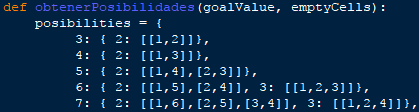
\includegraphics[width=.9\columnwidth]{obtenerPosibilidades.png}
        \caption{
                \label{fig:samplesetup}
                Parte de la función de poda
        }
\end{figure}

En la figura 4 se puede ver que la cantidad de combinaciones crece conforme el valor de la clave se incrementa, no obstante, cuando la clave se enctuentre entre 21 y 24 alcanza el valor máximo de posibles combinaciones, con diferentes valores de casillas consecutivas, las cuales varían en 23 posibles combinaciones. El límite que llega a alcanzar el valor de la clave es de 45, el cual posee una única combinación posible, que es la sumatoria del 1 al 9.\\
De lo anterior se puede decir que $O(obtenerPosibilidades(clave, celdas))$ se encuentra cuando el valor de la clave es 45 ó cuando el valor de la clave es 24 y la cantidad de celdas es el máximo para generar la suma de la clave, las cuales serían 6 celdas consecutivas. Entonces:

\[O(obtenerPosibilidades(45, 9))=46\]
\[O(obtenerPosibilidades(24, 6))=47\]

Por lo tanto $O(obtenerPosibilidades)=47$

\subsection{Backtracking}
Al momento de analizar las funcio\'{o}nes encargadas del backtraking, se debe de tomar en cuenta que el orden puede ser afectado por otras funci\'{o}nes, como por ejemplo las encargadas de la poda, sin embargo, al ser estudiadas en otra secci\'{o}n, no se contemplara el efecto que tengan en el orden del backtracking.\\
El kakuro tiene la particularidad de solo tener, por numero, 9 casillas vaci\'{a}s, por lo que el rango maximo de interaciones por numero a calcular es de 9.\ La funci\'{o}n backtrack, figura 4, busca la solucion con un maximo de 11 veces por el parametro "intentos" (maximo de veces que un mismo numero aparece en una lista de los posibles conjuntos) si no es que no ha encontrado una soluci\'{o}n, al analizarla obtenemos un orden $O((n*{11}*k))$ donde $k$ es la cantidad de veces que la recursividad necesiat evaluar por casilla, que a su vez se puede reducir a  $O((n*k))$ ,se tiene que tener en cuenta que backtrack llama a la funci\'{o}n meterEnMatriz, figura 5, por lo que es necesario el estudio de la funci\'{o}n meterEnMatriz.
\\
La funci\'{o}n meterEnMatriz entra en un while que puede tener dos duraciones, en el mejor caso una duraci\'{o}n de 9 (en el caso de ser una serie de 9 espacios en blanco sin ninguna intersecci\'{o}n) o de 15 como maximo de interaciones antes de que se requiera otro grupo de soluci\'{o}n (el cual se encarga la funci\'{o}n backtrack), por lo que el orden de la funci\'{o}n esta dada por $O(15)$ al ser 15 el maximo entre (9,15).\\ Con lo anterior, podemos deducir que la O grande del backtracking, como un todo, seria de $O(n*k)*O(C)$, con C siendo la constante 15 de la O grande de la funci\'{o}n meterEnMatriz, a lo que termina siendo $O(n*k)$
\begin{figure}[H] 
	\centering 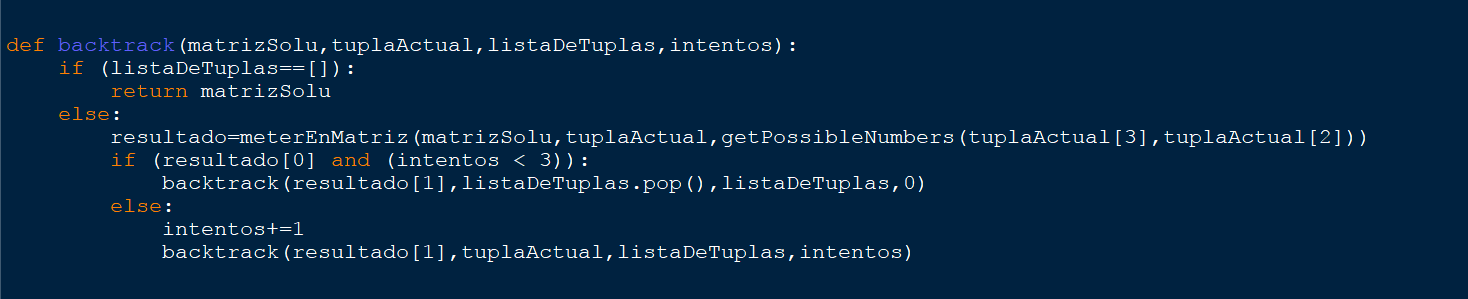
\includegraphics[width=1\columnwidth]{backtrack_parte1.png}
	\caption{
		\label{fig:samplesetup}
		Función de Backtrack
	}
\end{figure}
\begin{figure}[H] 
	\centering 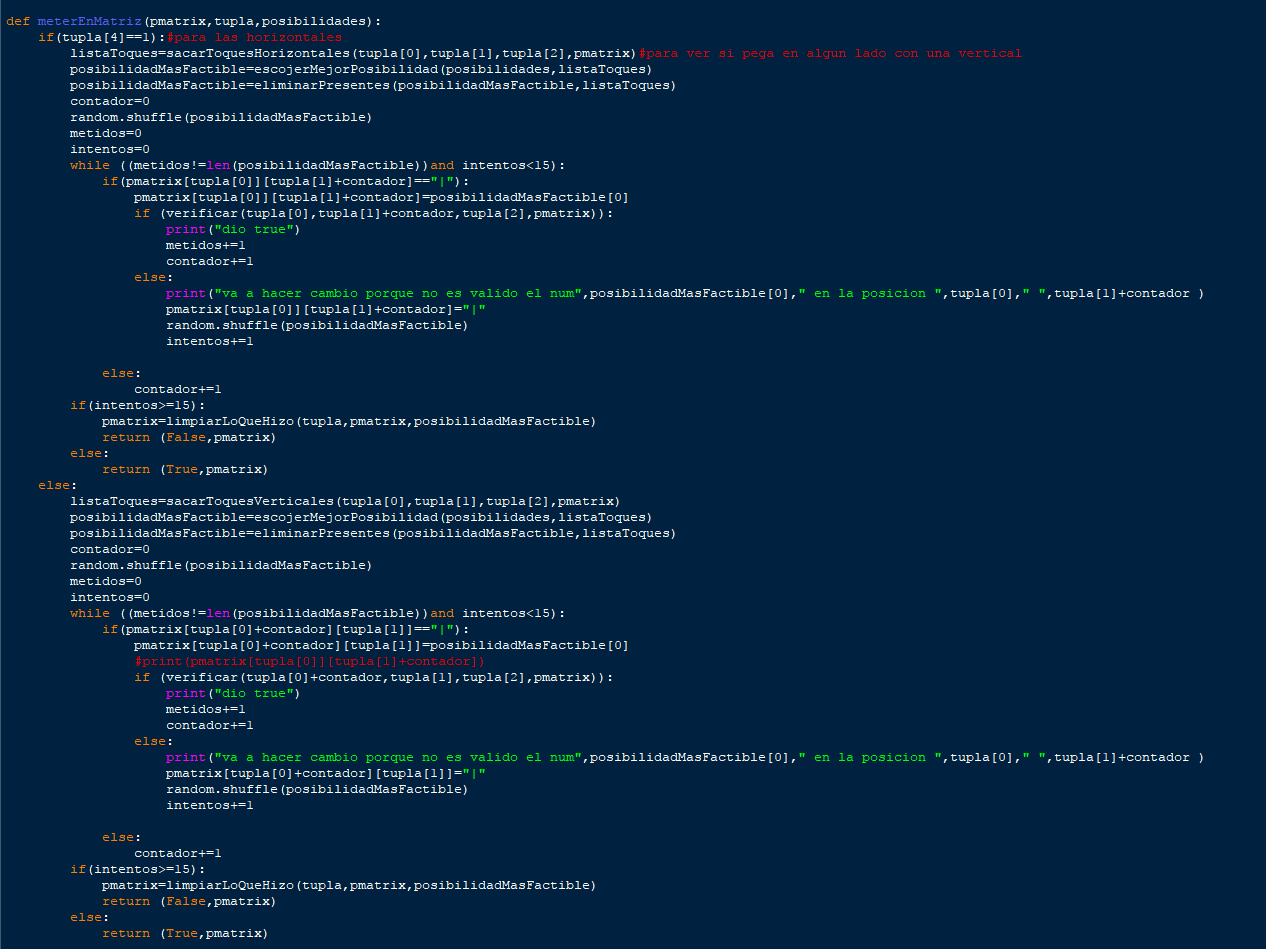
\includegraphics[width=1\columnwidth]{backtrack_parte2.png}
	\caption{
		\label{fig:samplesetup}
		Función de meterEnMatriz
	}
\end{figure}

\section{Experimentos	y	discusión}
\subsection{Hilos}
La utilizaci\'{o}n de los hilos en la busqueda de la soluci\'{o}n de un kakuro en la teor\'{\i}a, parece fiable, pero a la hora de aplicarlos en la soluci\'{o}n crea problemas en la soluci\'{o}n, usualmente crea resultados invalidos en el kakuro, como lo son numeros repetidos en filas y columnas, o bien , sumas que dan respuesta correcta en una direcci\'{o}n pero no es su opuesta inmediata.En la figura 7 se muestra el codigo utilizado en la aplicaci\'{o}n de los hilos(deamon).\ El poder paralelizar el calculo de las posibilidades de cada grupo de casillas aumenta el tiempo de calculo, pero al multiples estar trabajando sobre una misma matriz, provoca las inconsistencias anteriormente mencionadas.
\begin{figure}[h] 
	\centering 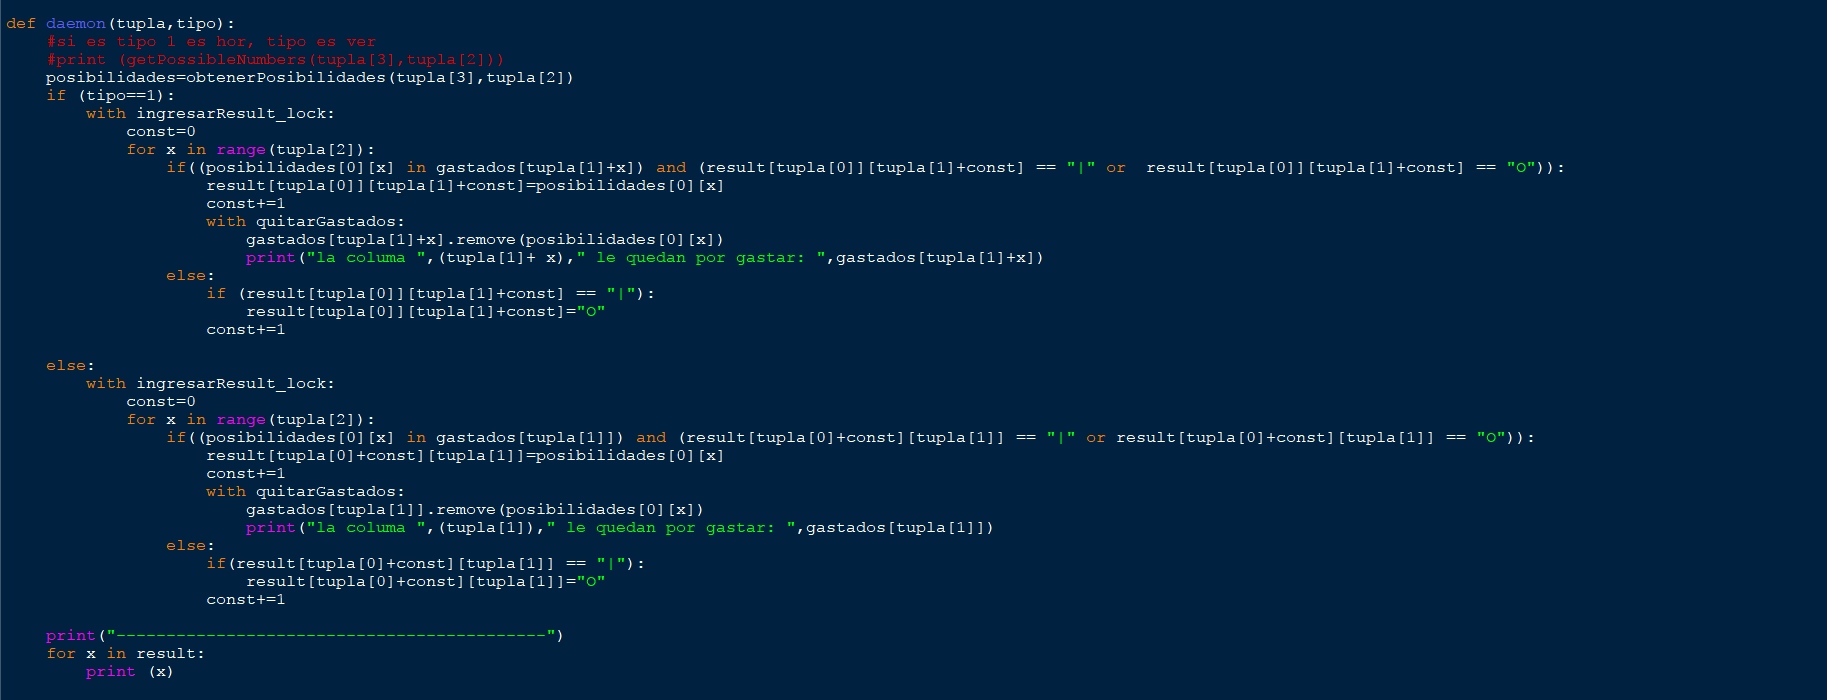
\includegraphics[width=1\columnwidth]{hilos.png}
	\caption{
		\label{fig:samplesetup}
		Función de deamon (Hilos)
	}
\end{figure}

\subsection{Forks}
Los forks son una herramienta que ayuda a mejorar considerablemente el rendimiento del programa. Su funcionamiento consiste en la copia idéntica de un proceso que se está llevando a cabo, el cual será el proceso hijo, incluyendo todas las variables que se declararon antes de la bifurcación del proceso, a excepción de la que guardará el resultado una vez que termine el proceso hijo y su ejecución continua en la línea inmediata después de la duplicación del proceso.\\
La implementación de este método no pudo ser implementada en este proyecto, sin embargo pudo haber sido de mucha utilidad a la hora de realizar los procesos, mejorando los tiempos de respuestas realizando múltiples tareas a la vez.

\subsection{Experimentos}
Utilizando distintas dimensiones y múltiples pruebas se obtuvo un resultado en el promedio que tarda resolviendo los kakuros de distintos tamaños y se obtuvo los siguientes resultados:\\

\begin{figure}[h] 
	\centering 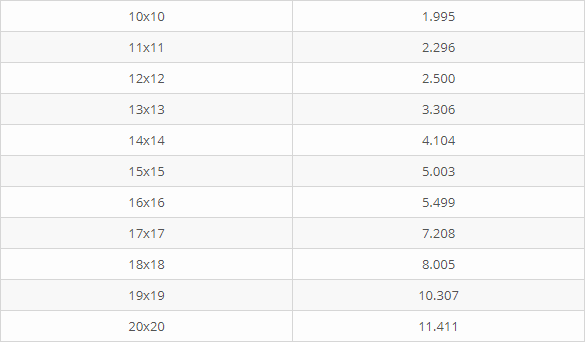
\includegraphics[width=1\columnwidth]{valores.png}
	\caption{
		\label{fig:samplesetup}
		Tamaños utilizados y tiempo en segundos obtenidos
	}
\end{figure}

\begin{figure}[h] 
	\centering 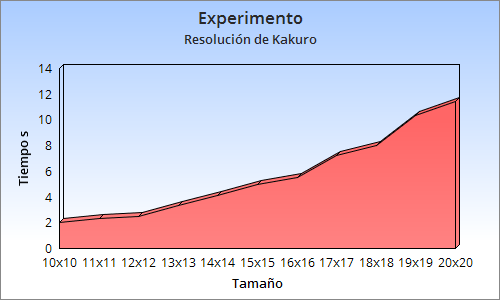
\includegraphics[width=1\columnwidth]{grafico.png}
	\caption{
		\label{fig:samplesetup}
		Representación gráfica
	}
\end{figure}

\end{document}